\chapter{Comparing Devices}
\section{Research Task}
The core application allows easy access to meassurements from multiple devices in a csv format. This enables researchers to analyse the data to answer research questions. As a supplementary project task, a data analysis was performed to answer the following research question: "Do devices used (Withing scanwatch and Oura gen 2 ring) produce significantly different measurements for common fields?" Importantly, this is not the same as answering: "Are devices used accurate?", as that would require a much more rigorous study; that would require ground-truth measurements for every day, which are hard to acquire in practice, as those machines are expensive, non-mobile, require technician, etc. So it would be a very expensive, industry-level study, which is out of scope for this project. Instead, the precision of the differences in device measurements is examined rather than an individual device accuracy. 
\section{Data}
There are 60 days of my own personal data from both devices for every day. I always wore both devices at the same time, never one device but not the other; Both devices were configured properly - such as indicating correct weight in both apps every week and setting reference values for heart-rates to automatic. That means that data from devices is directly comparable. It is only 60 days because I acquired the ring later in the year than the watch, around the end of December, so earlier data could not be used as there is no corresponding ring data. Lastly, only common measurements were used. Withings watch did not measure REM Sleep, so that field was deleted from the Oura rows for the analysis.
% TODO technologies in backend.
\section{Exploration}
Python with pandas, numpy and statsModels were used for analysis. To explore the dataset, Bland-Altman plot was used on various common measurements. The difference in measurements for the same date is calculated by: $\text{Oura[property]} - \text{Withings[property]}$, meaning that negative values mean that Oura ring's measurement was lower.
\begin{figure}
    
    \centering
    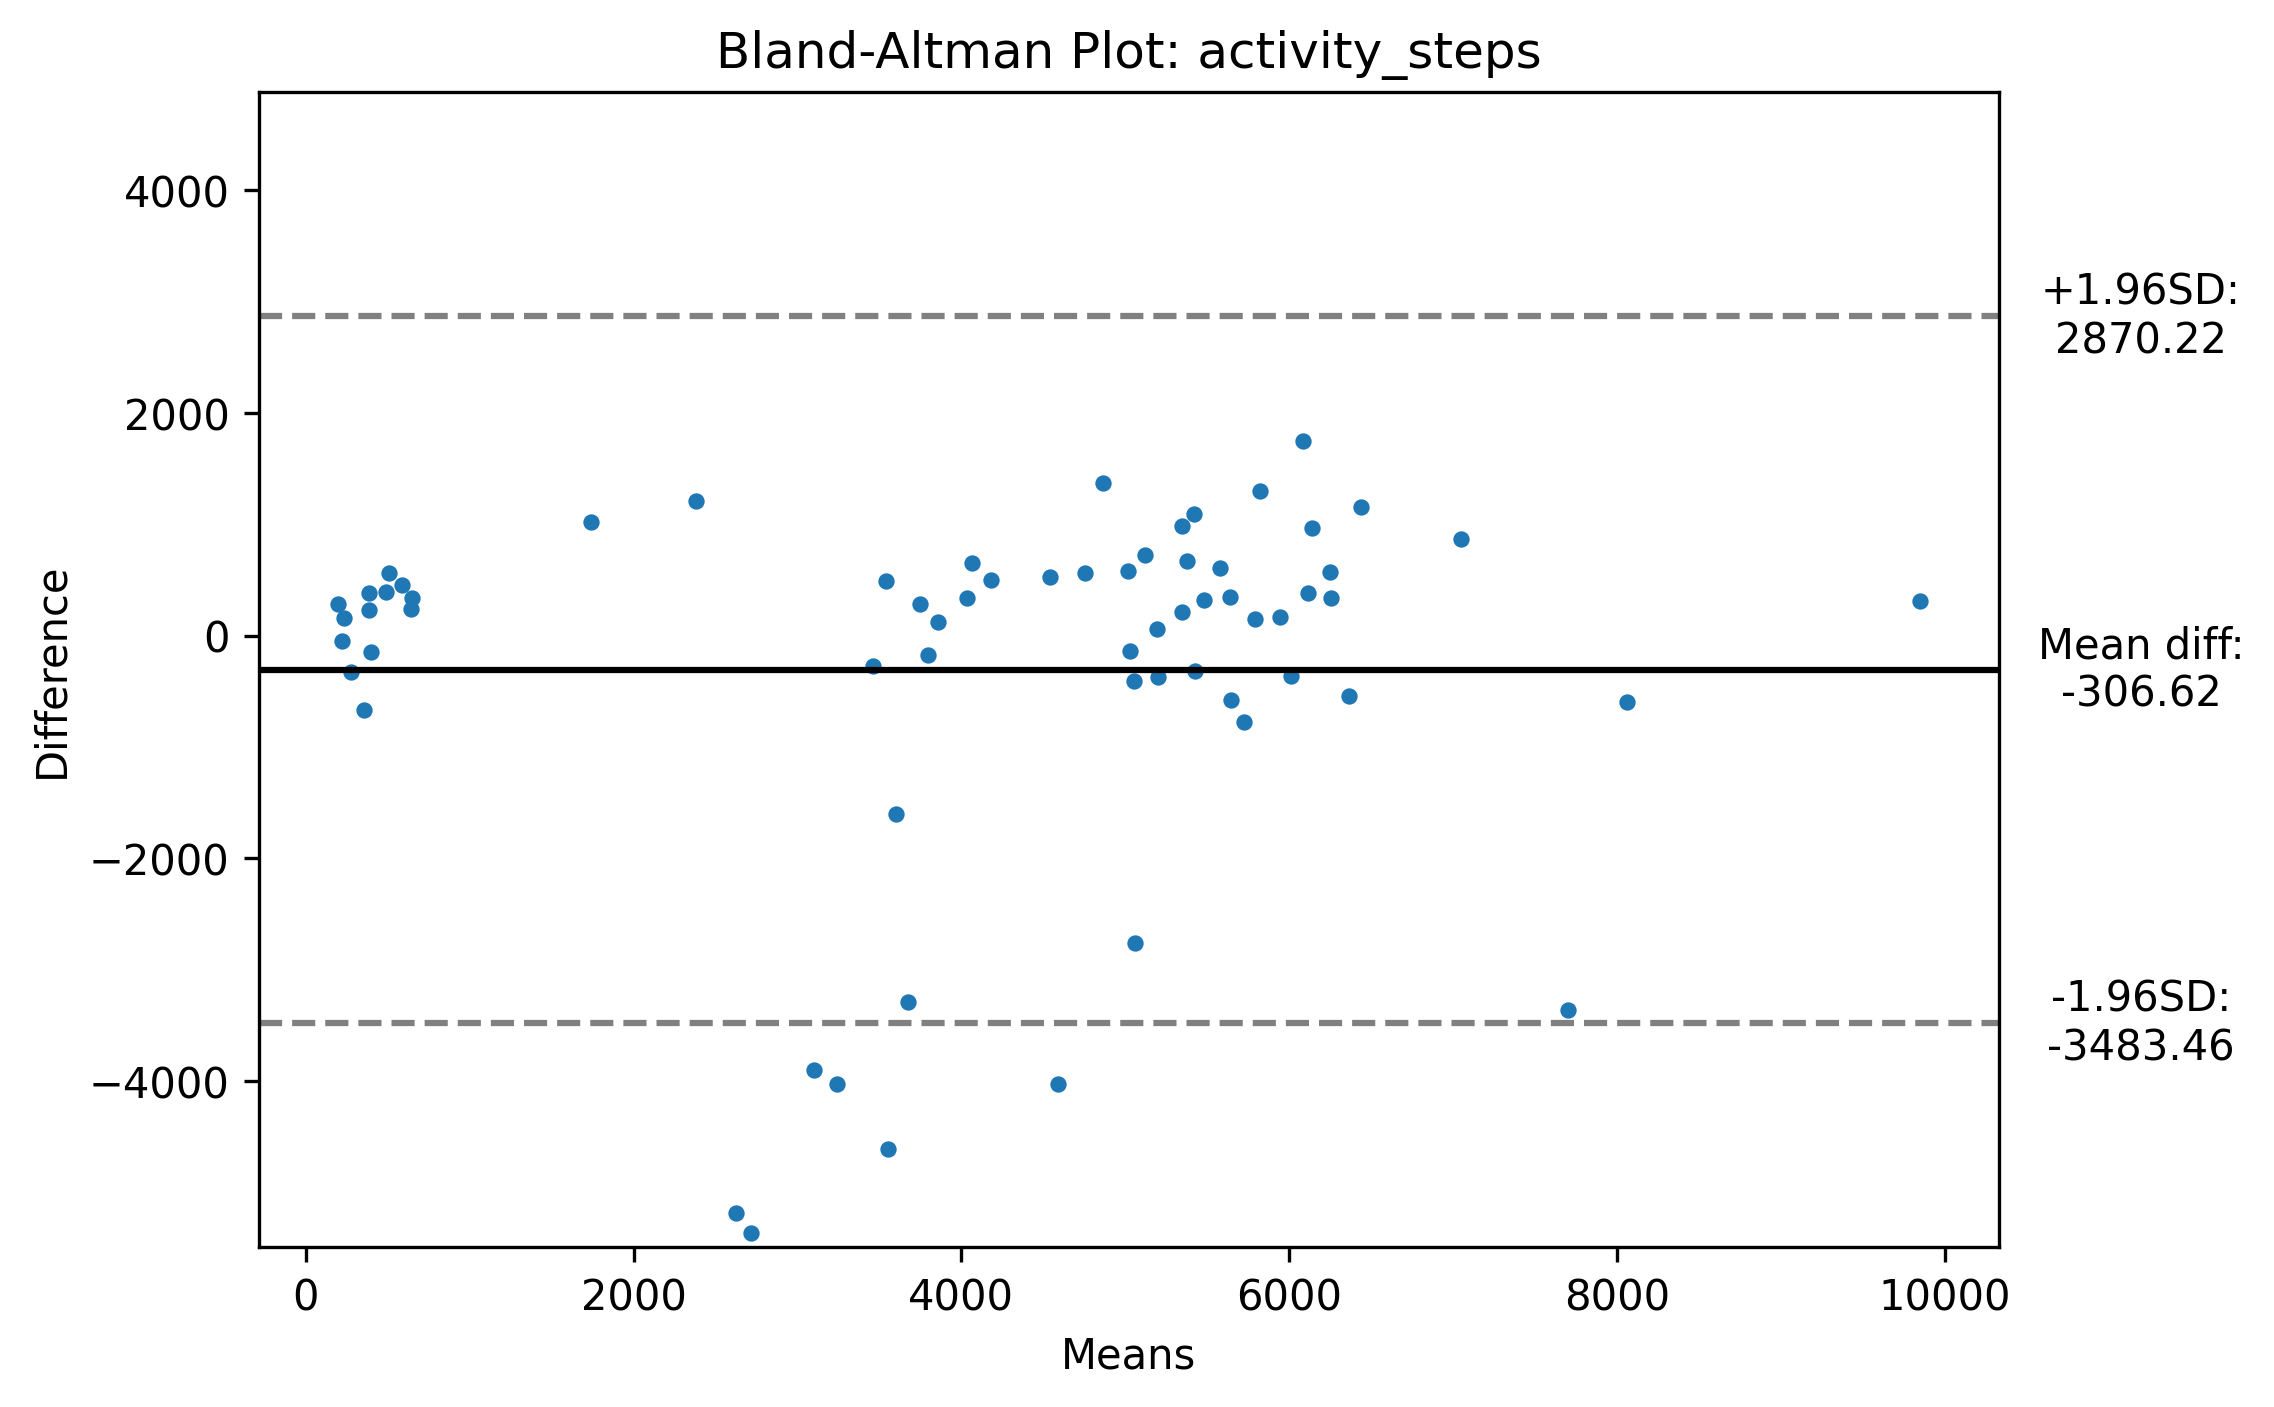
\includegraphics[width=\textwidth,keepaspectratio]{../images/bland_altman_steps.png}
    \caption{Bland-Altman Plot for Steps}
    \label{fig:blandAltmanSteps}
    
\end{figure}
\begin{figure}
    
    \centering
    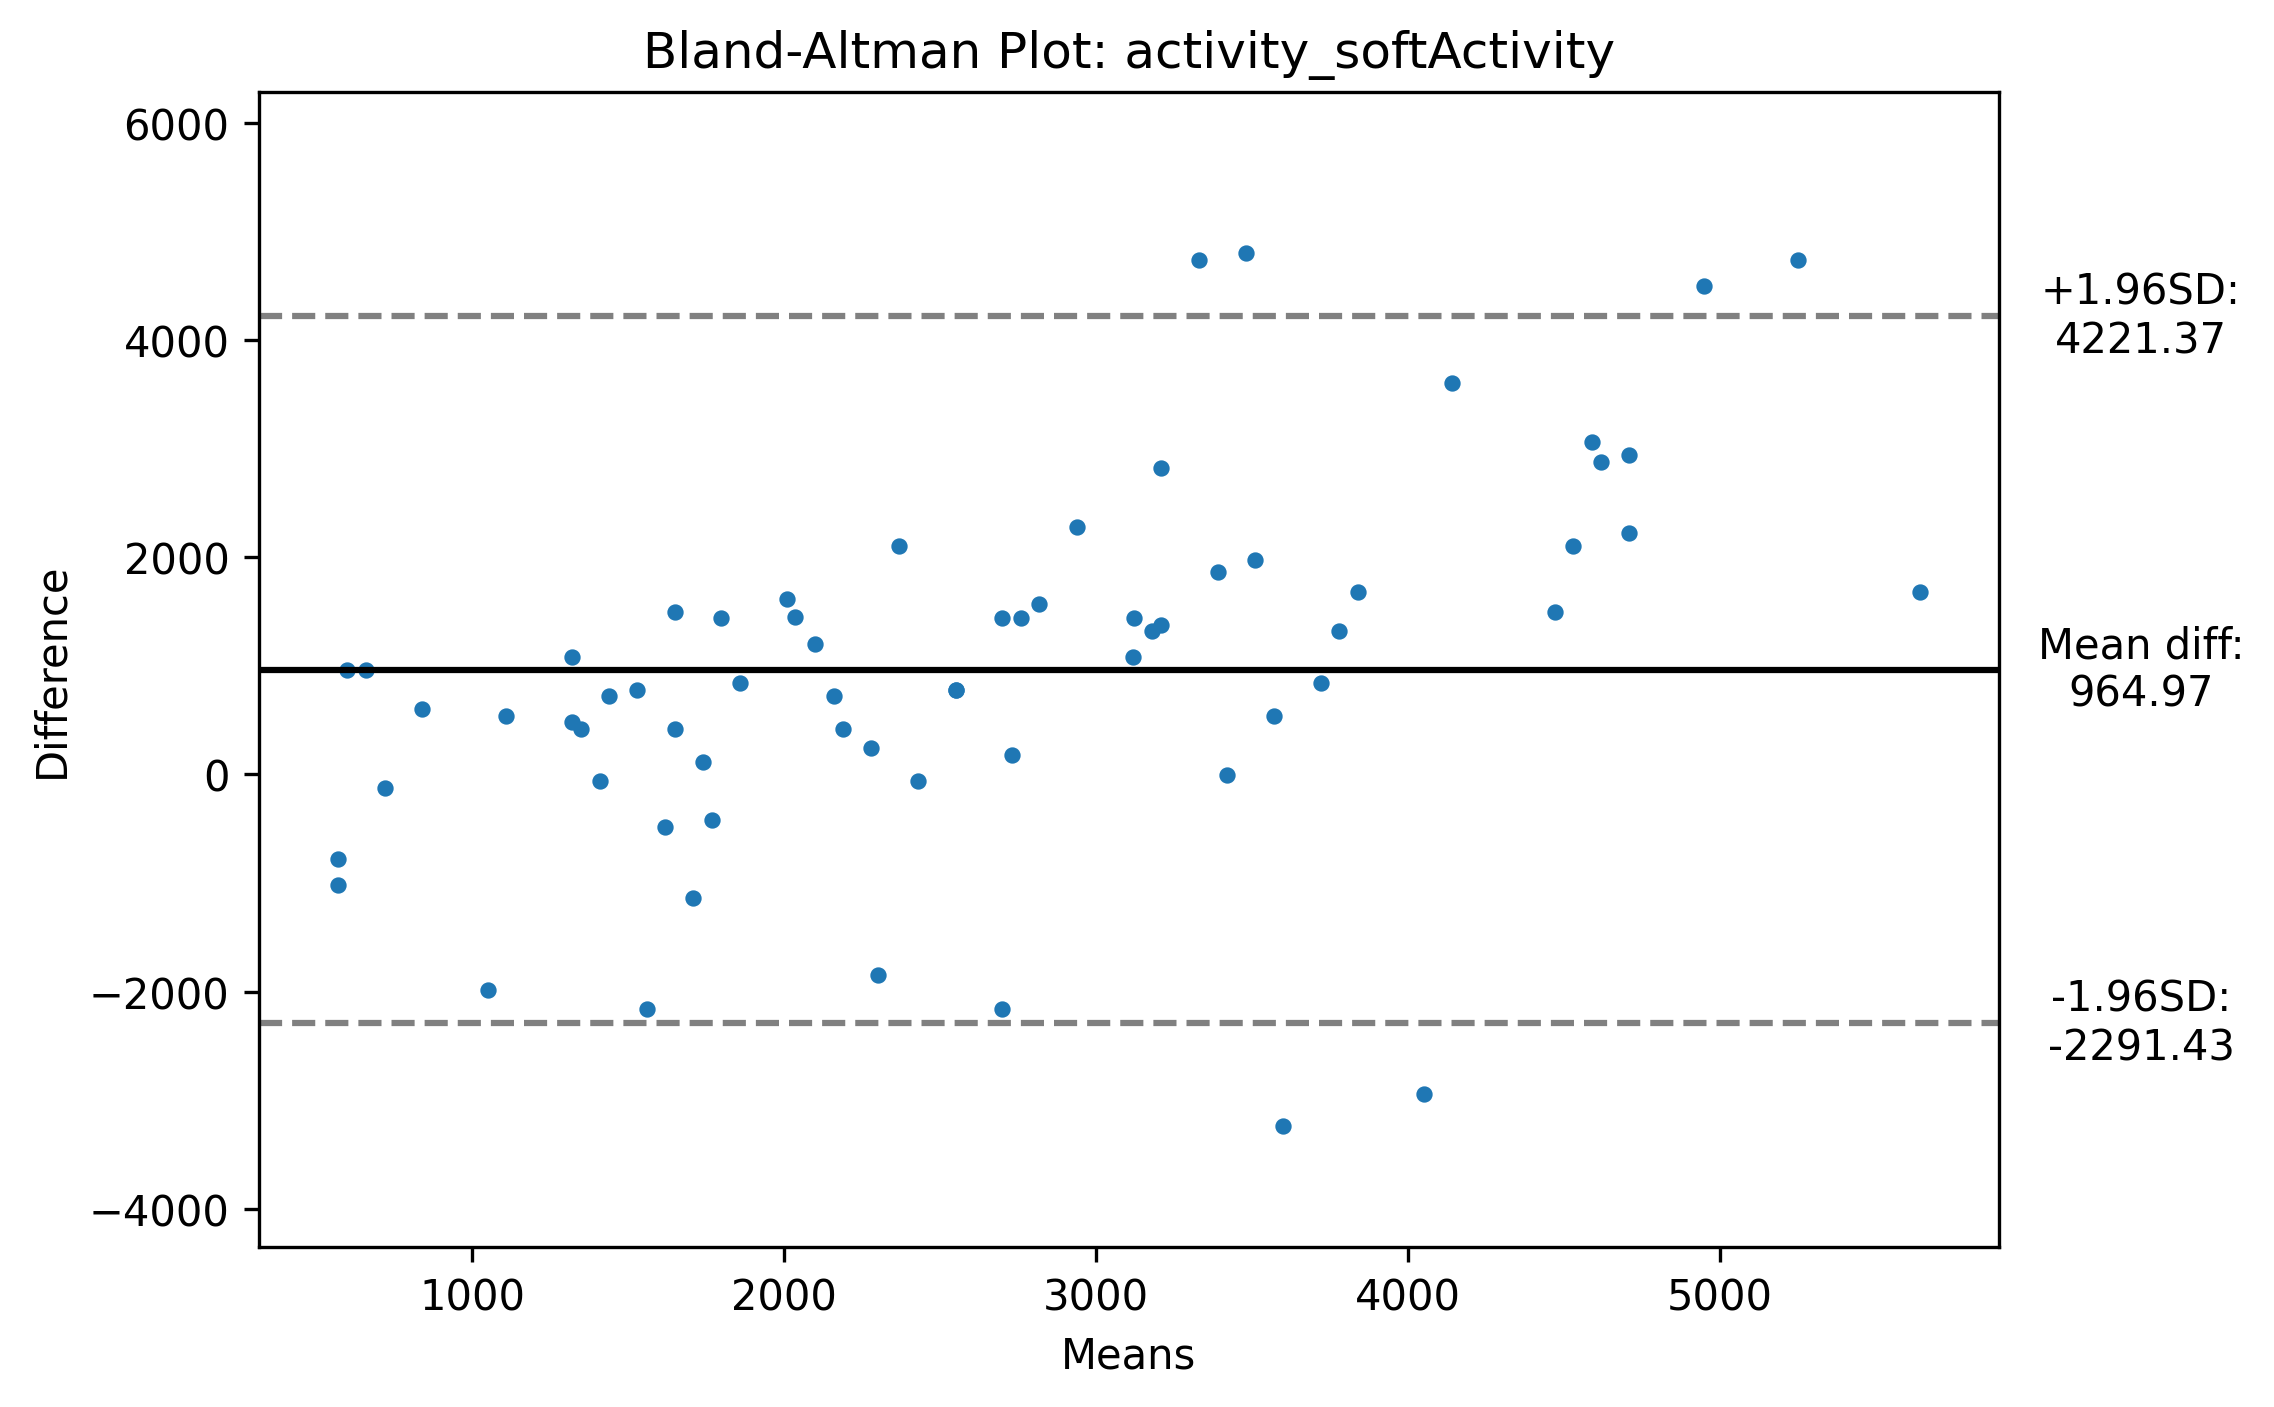
\includegraphics[width=\textwidth,keepaspectratio]{../images/bland_altman_softActivity.png}
    \caption{Bland-Altman Plot for Soft Activity Seconds}
    \label{fig:blandAltmanSoftActivity}
    
\end{figure}
